\documentclass[main.tex]{subfiles}
\begin{document}
\appendix
\chapter{FIN Scene Results}
\setcounter{page}{\thepage-1}
\label{app:fin}

\begin{figure}[H]
    \centering
    \def\svgwidth{0.7\textwidth}
    \input{images/dynconf_crop.pdf_tex}
    \caption[Time Results Conference Room Scene]{Time spent in pre-processing $t_{pre}$, plane detection $t_{calc}$, post-processing
        $t_{post}$, and total calculation time $t_{tot}$ of the \textit{conference room} scene, and point cloud size of each time frame.
        Note that both y-axes are scaled logarithmically to the base of ten. \textit{Time Frames} are defined in Subsection~\ref{subsec:metrics}.}
    \label{fig:dynconf}
\end{figure}

\begin{figure}[H]
    \centering
    \def\svgwidth{0.7\textwidth}
    \input{images/dynhall_crop.pdf_tex}
    \caption[Time Results Hallway Scene]{Time spent in pre-processing $t_{pre}$, plane detection $t_{calc}$, post-processing
        $t_{post}$, and total calculation time $t_{tot}$ of the \textit{hallway} scene, and point cloud size of each time frame.
        Note that both y-axes are scaled logarithmically to the base of ten. \textit{Time Frames} are defined in Subsection~\ref{subsec:metrics}.}
    \label{fig:dynhallway}
\end{figure}

\begin{figure}[p]
    \centering
    \def\svgwidth{0.7\textwidth}
    \input{images/dynoffice_crop.pdf_tex}
    \caption[Time Results Office Scene]{Time spent in pre-processing $t_{pre}$, plane detection $t_{calc}$, post-processing
        $t_{post}$, and total calculation time $t_{tot}$ of the \textit{office} scene, and point cloud size of each time frame.
        Note that both y-axes are scaled logarithmically to the base of ten. \textit{Time Frames} are defined in Subsection~\ref{subsec:metrics}.}
    \label{fig:dynoff}
\end{figure}

\chapter{FIN Dataset Scenes}
\label{app:fin-scenes}


\begin{figure}[H]
    \centering
    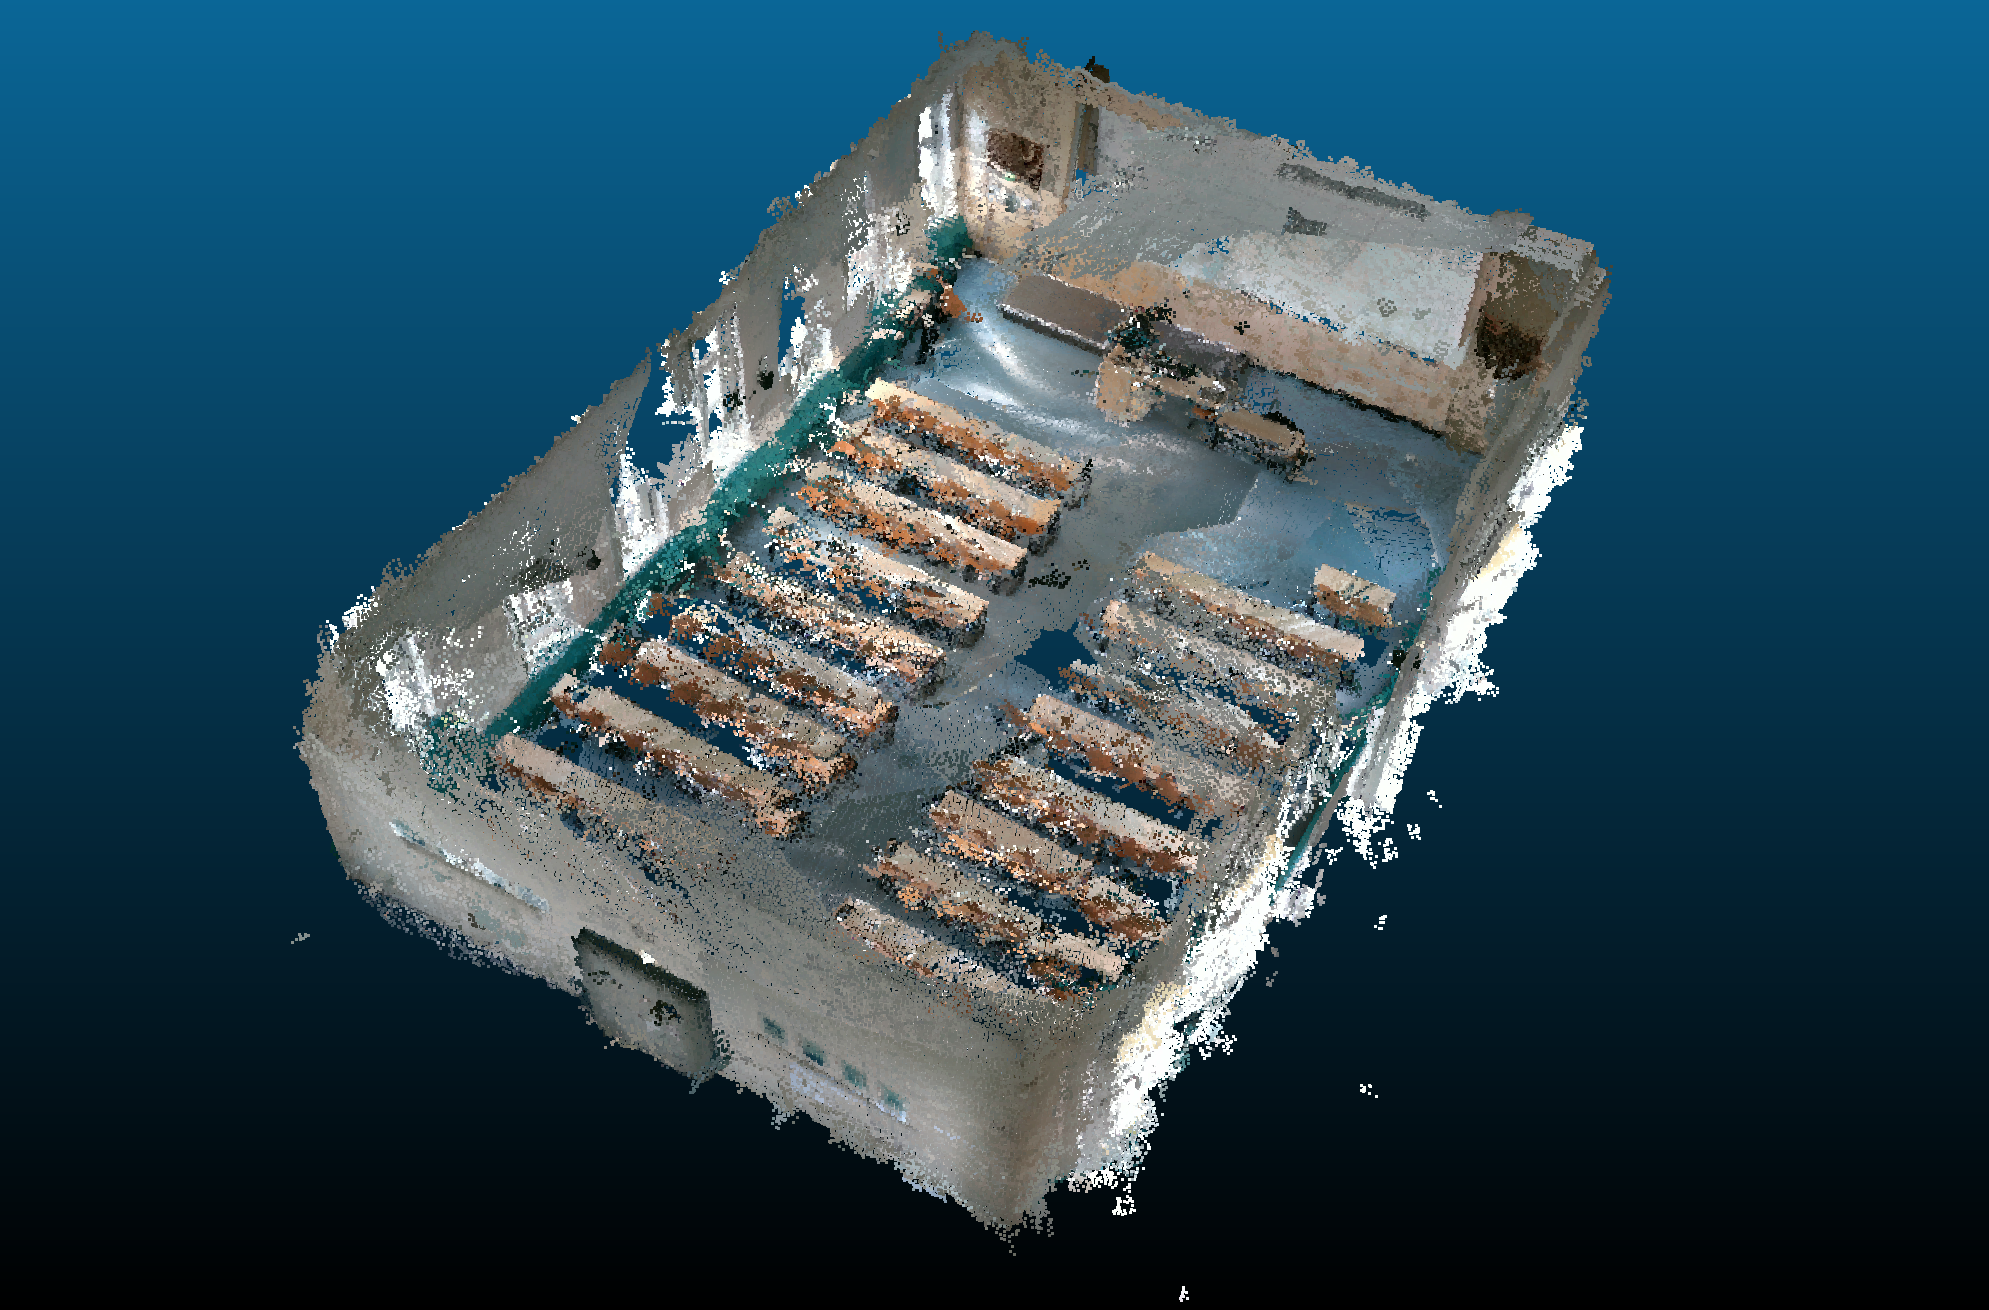
\includegraphics[width=0.9\textwidth]{images/307.png}
    \caption[FIN Auditorium Scene]{Full-size view of the hallway scene of the FIN dataset.}
    \label{fig:fin307-app}
\end{figure}
\begin{figure}[H]
    \centering
    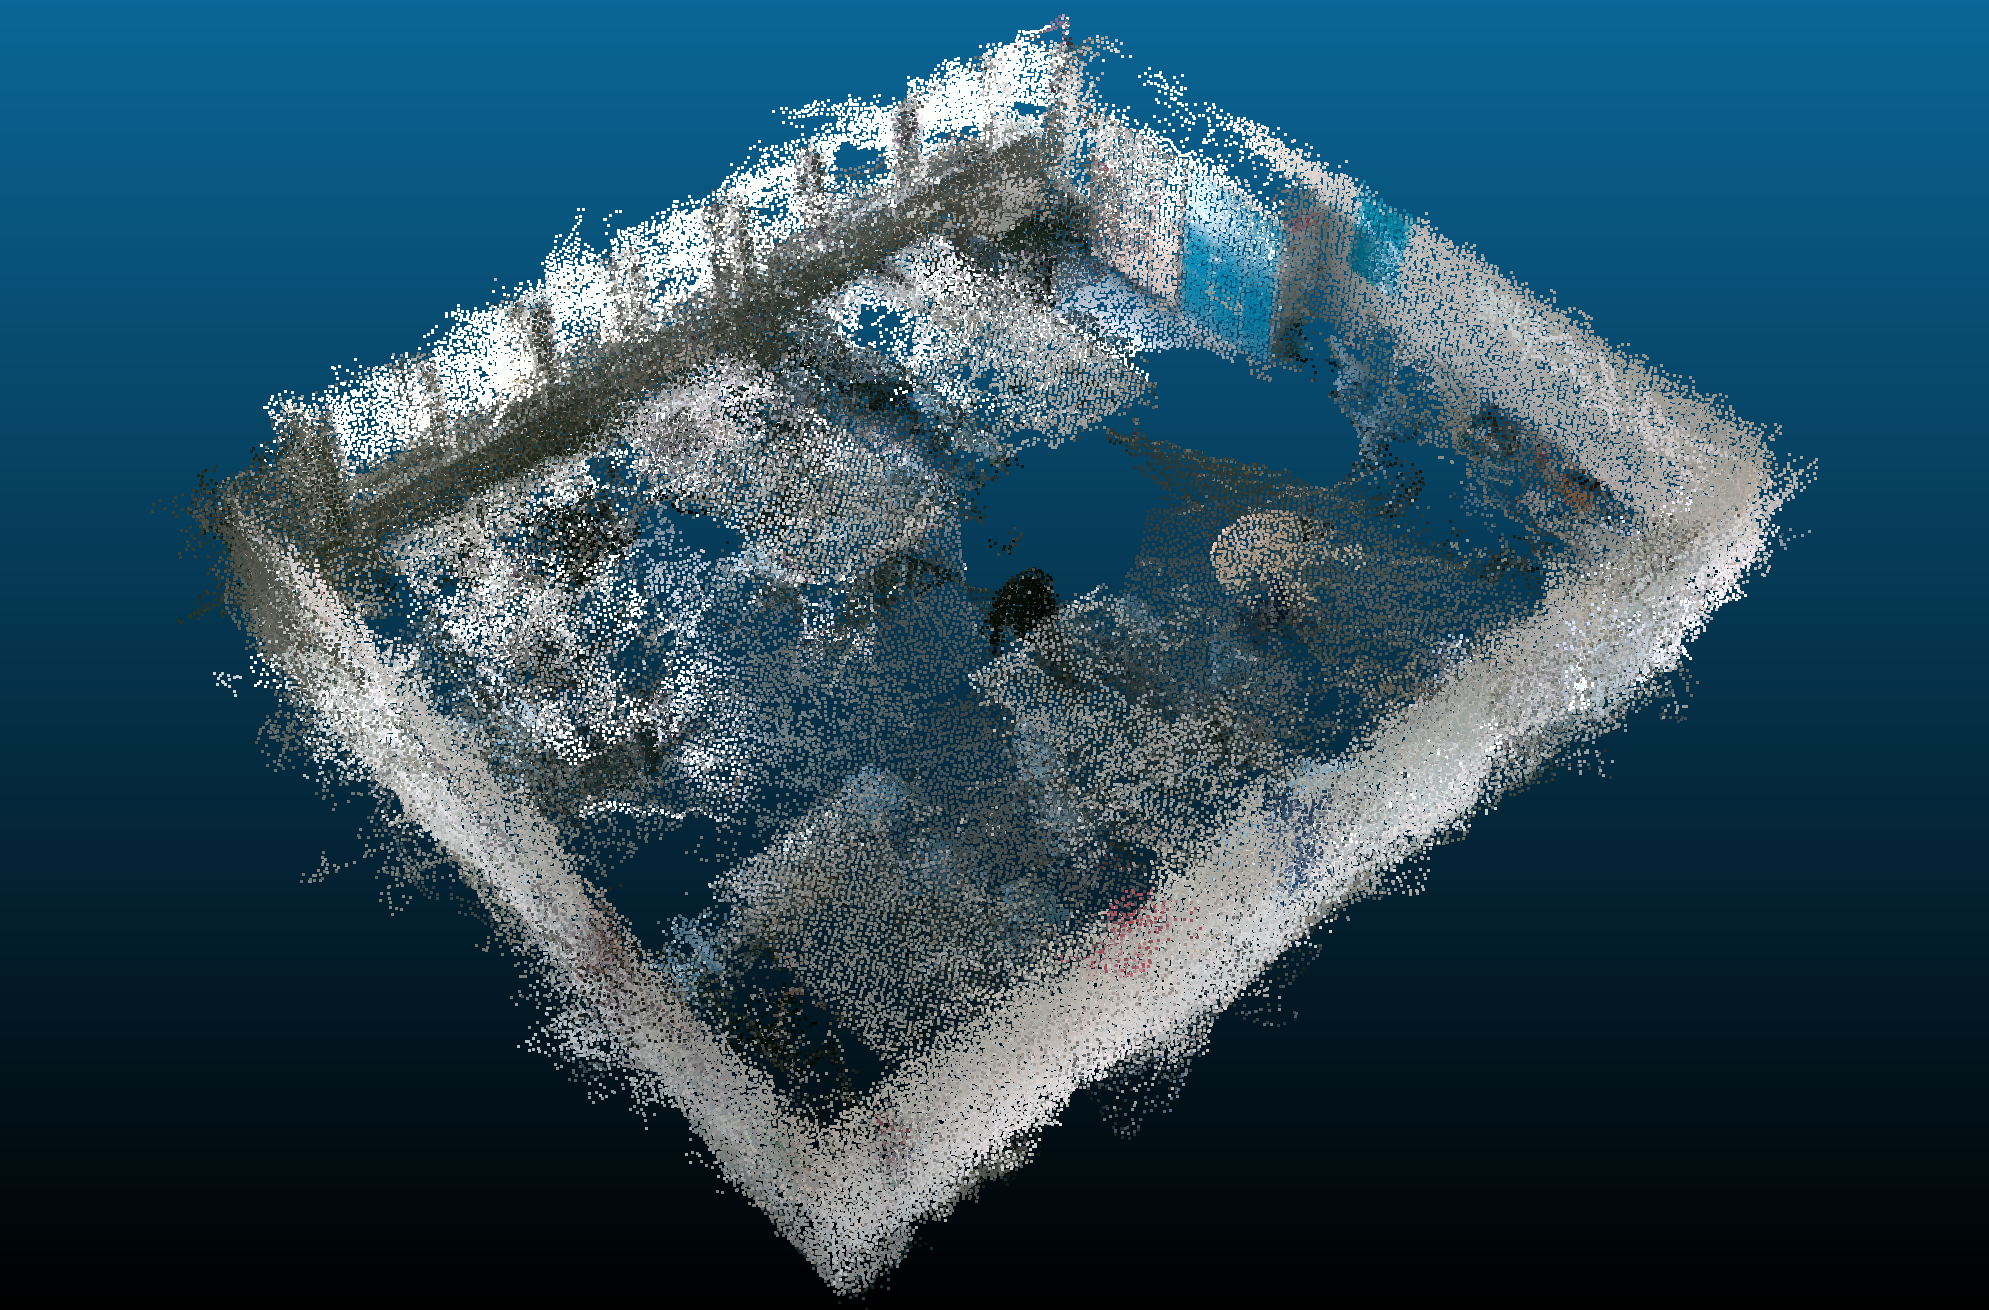
\includegraphics[width=0.9\textwidth]{images/333.png}
    \caption[FIN Conference Room Scene]{Full-size view of the conference room scene of the FIN dataset.}
    \label{fig:fin333-app}
\end{figure}
\begin{figure}[H]
    \centering
    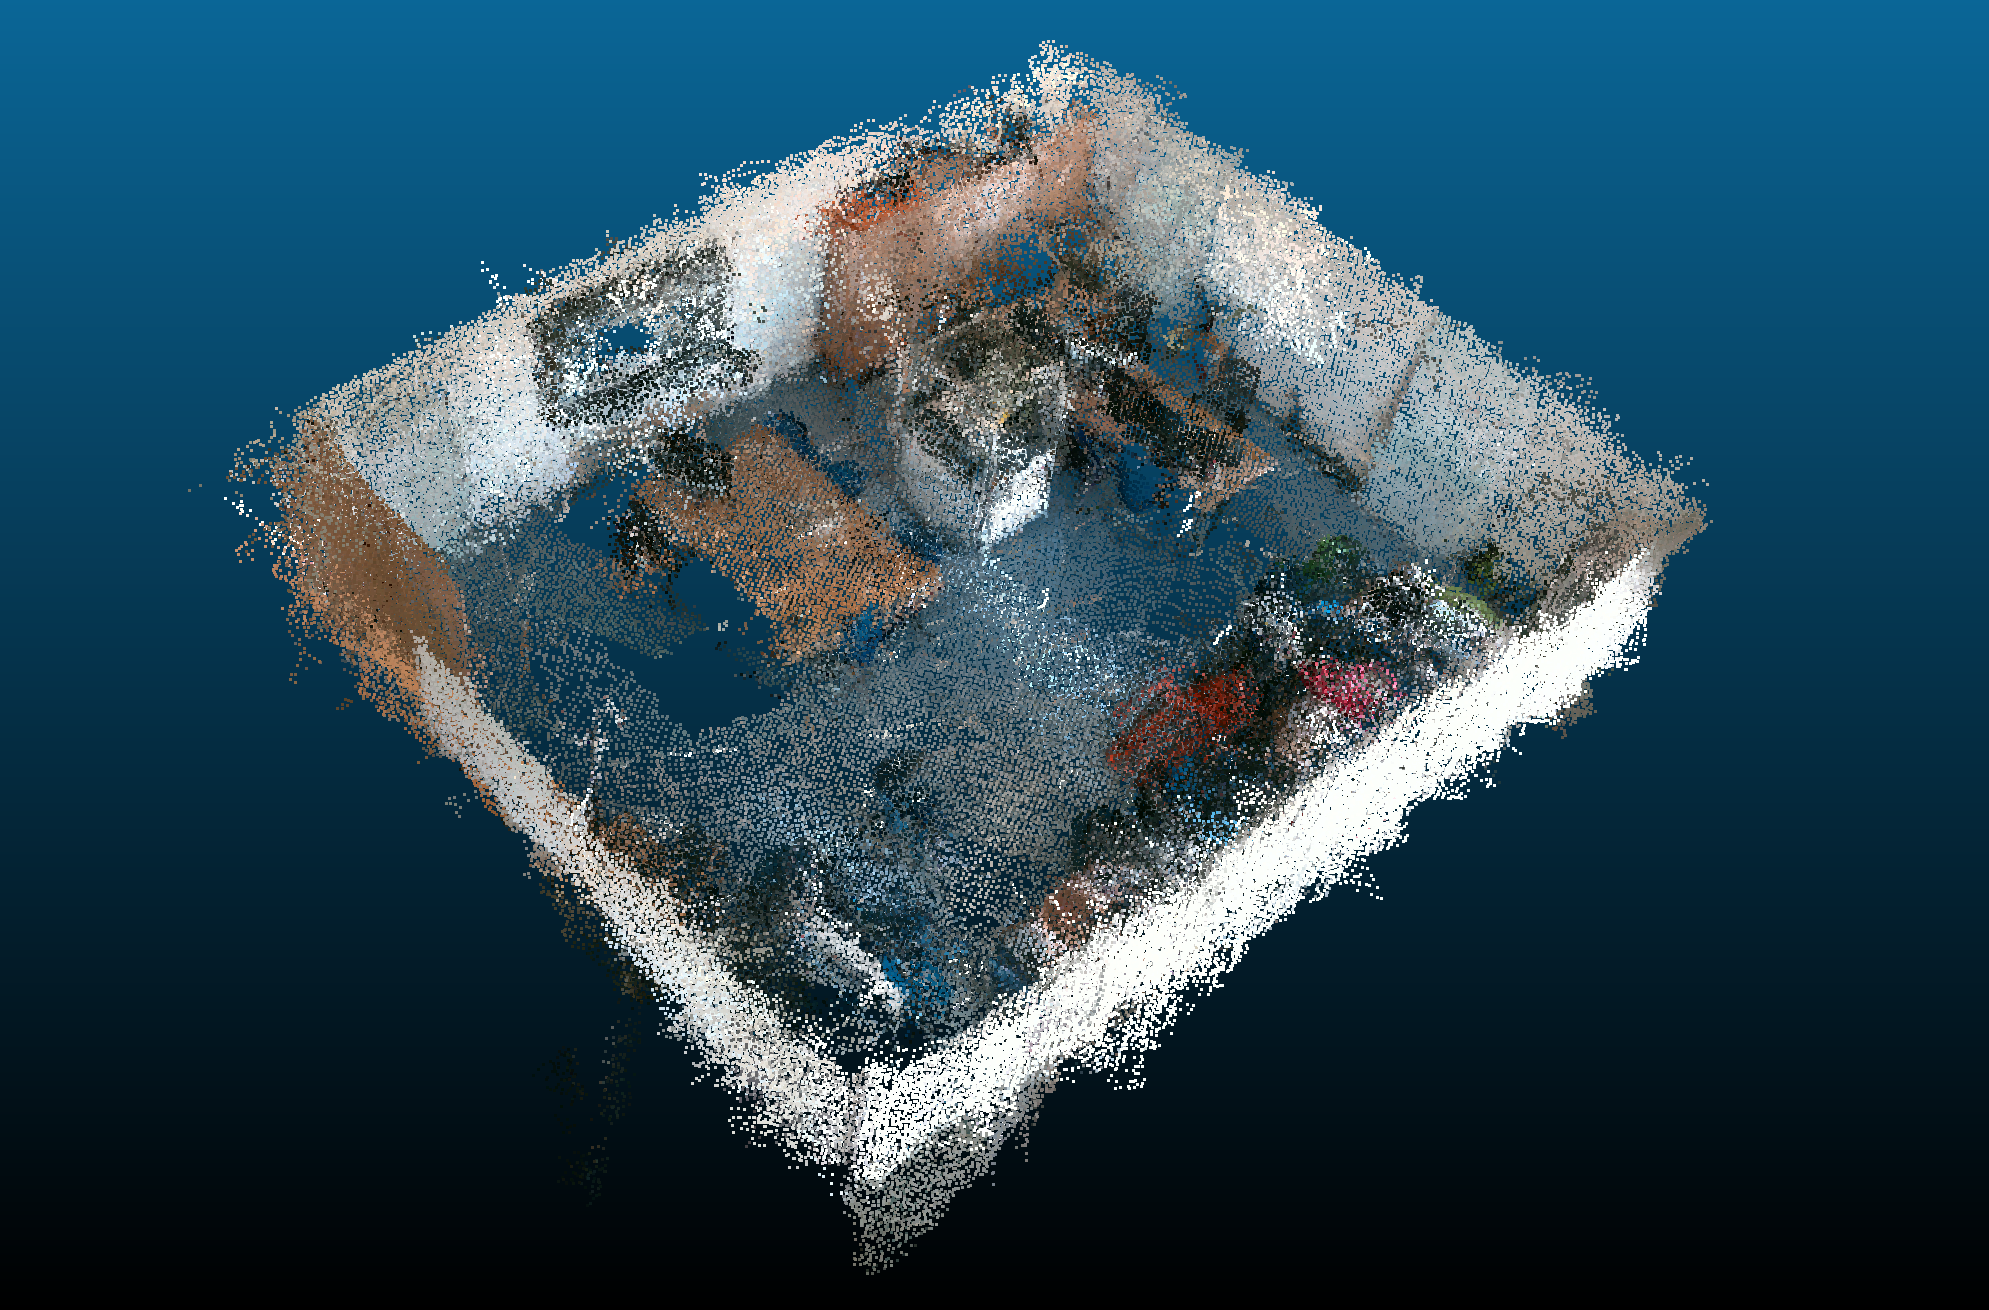
\includegraphics[width=0.9\textwidth]{images/425.png}
    \caption[FIN Office Scene]{Full-size view of the office scene of the FIN dataset.}
    \label{fig:fin425-app}
\end{figure}
\begin{figure}[H]
    \centering
    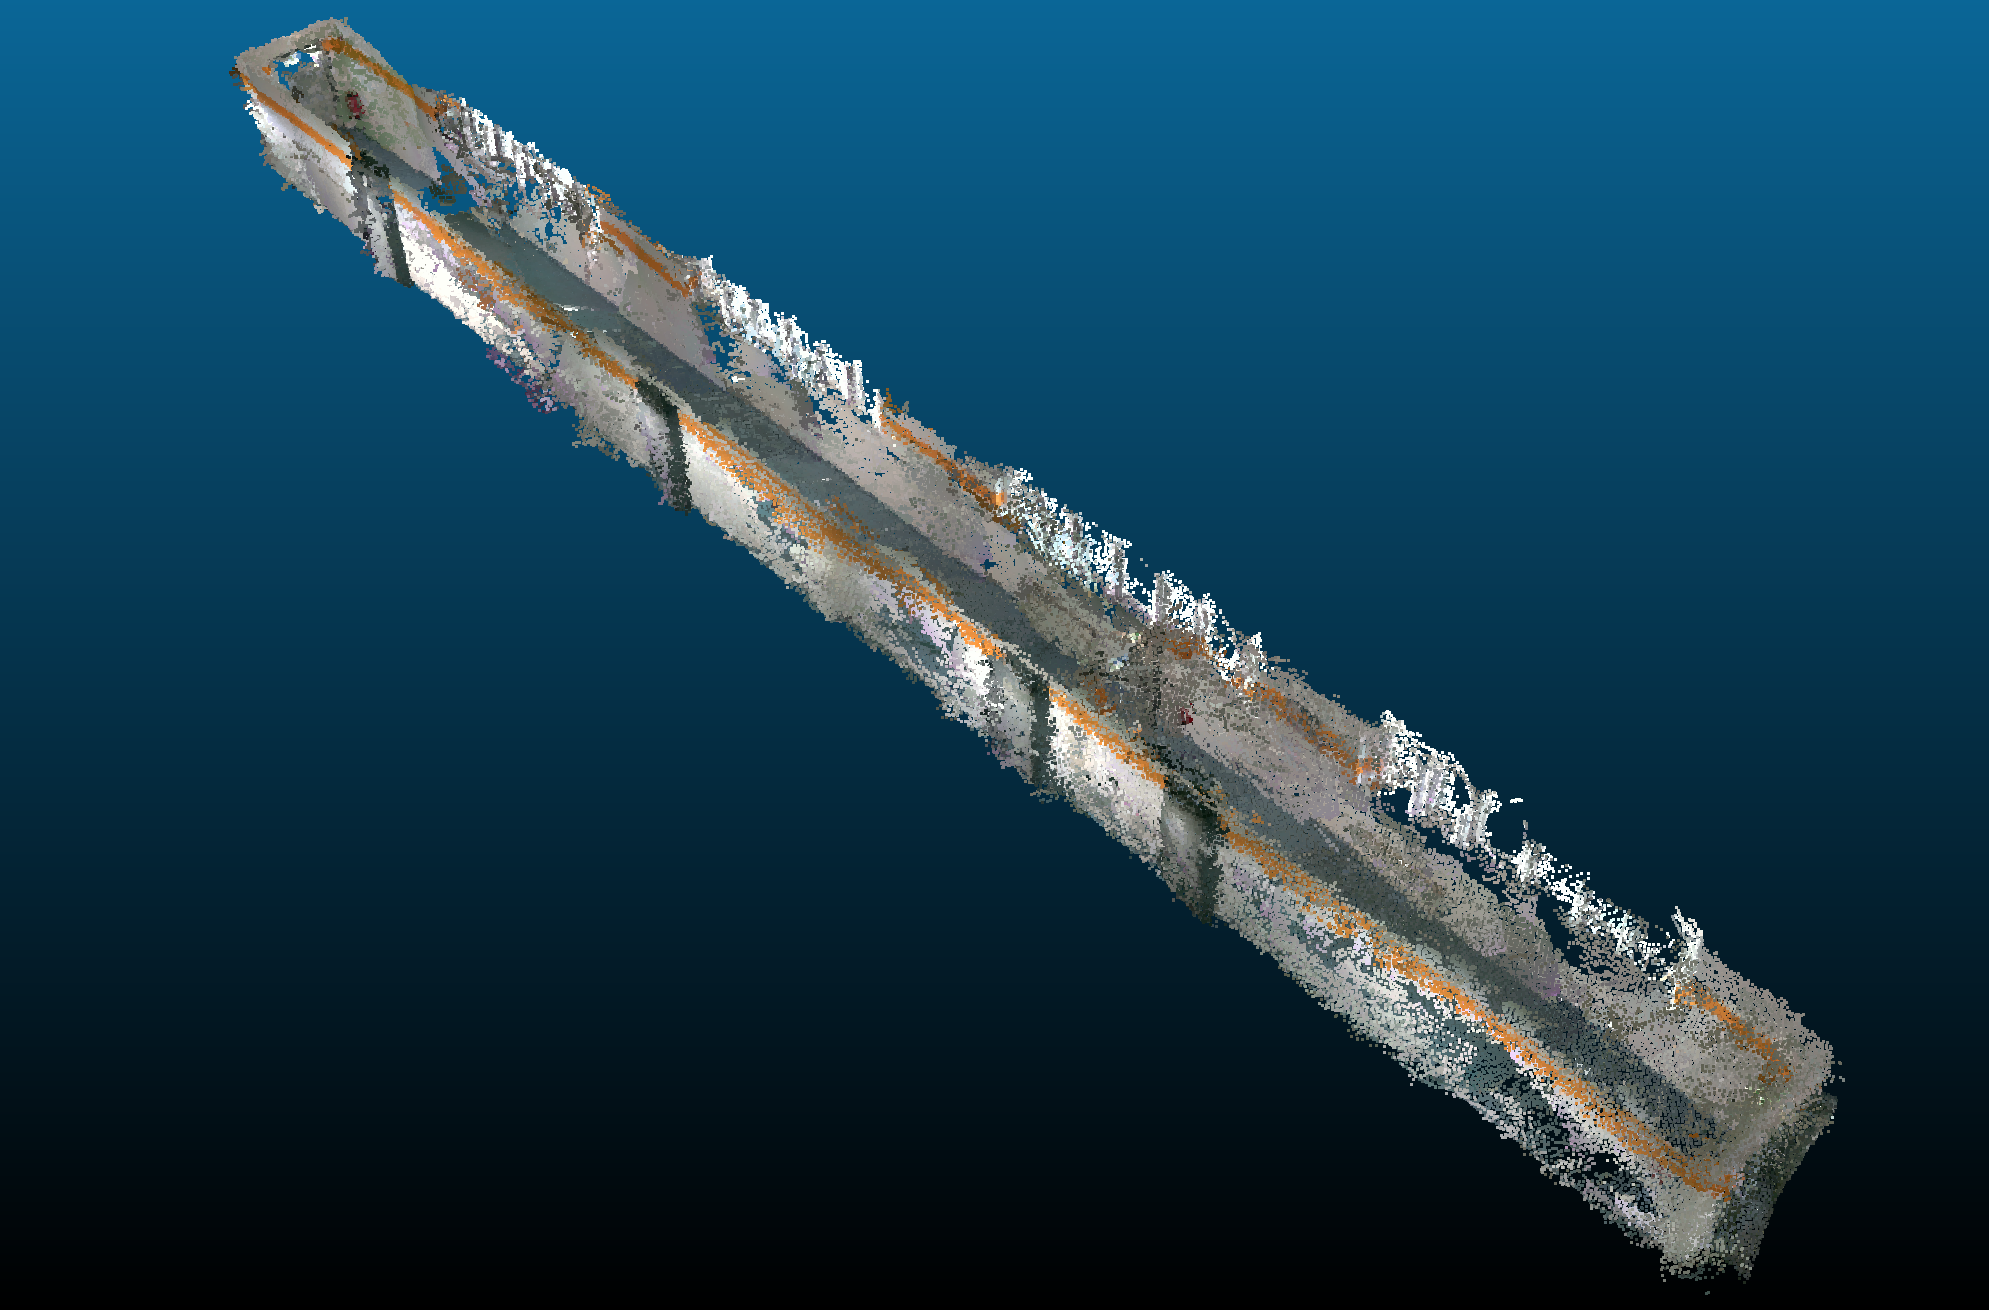
\includegraphics[width=0.9\textwidth]{images/hallway.png}
    \caption[FIN Hallway Scene]{Full-size view of the hallway scene of the FIN dataset.}
    \label{fig:finhw-app}
\end{figure}


\end{document}